\documentclass[12pt]{article}

\title{\vspace{-1em}PHYS 163a HW 3}
\author{Michael Cardiff}
\date{\today}

%% science symbols 
\usepackage{amsmath}
\usepackage{amssymb}
\usepackage{physics}
\usepackage{slashed}

%% general pretty stuff
\usepackage{bm}
\usepackage{enumitem}
\usepackage{float}
\usepackage{graphicx}
\usepackage[margin=1in]{geometry}
\usepackage[labelfont=bf]{caption}
\usepackage{tikz}

% figures
\graphicspath{ {./figs/} }

\renewcommand{\L}{\mathcal{L}}

\newcommand{\D}{\partial}
\newcommand{\munu}{{\mu\nu}}
\newcommand{\sla}[1]{\slashed{#1}}
\newcommand{\PB}[2]{\{#1,#2\}_{PB}}
\newcommand*\circled[1]{\tikz[baseline=(char.base)]{
    \node[shape=circle,draw,inner sep=2pt] (char) {#1};}}

\begin{document}
\maketitle

\section{Phase Space of a Harmonic Oscillator}
The Hamiltonian used here replaces $x\to q$:
\begin{align*}
  H=\frac{p^2}{2m}+\frac12kq^2
\end{align*}
\subsection{Phase Space Trajectory}
The point of a harmonic oscillator is that the position oscillates, and since momentum is proportional to the derivative of position, so will the momentum, in general this produces an ellipse in phase space:
\begin{figure}[H]
  \centering
  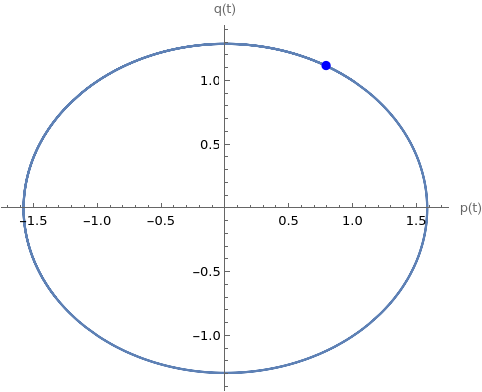
\includegraphics[width=4.0in]{phase1.png}
  \caption{Example Harmonic Oscillator Phase Space}
\end{figure}
Where the blue point is the initial condition $\{p_0,q_0\}$.
% \newpage
\subsection{Energy Condition}
Unlike the previous problem, this is technically only one constraint, so instead of a specific trajectory, we will get a region of possible trajectories. The semimajor and semiminor axes are changed by the energy, so it is a ring shaped region, and any path staying in between the region is valid:
\begin{figure}[H]
  \centering
  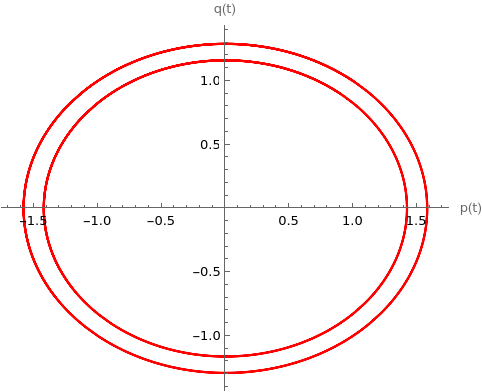
\includegraphics[width=9.0cm]{phase2.png}
  \caption{Harmonic Oscillator Phase Space with Energy Constraint}
\end{figure}
The inner ring would represent energy $E$ and the outer one would represent $E+\delta E$.

Some example trajectories are on the plot below, they can get a bit crazier, but I do not want to spent the effort to draw them:
\begin{figure}[H]
  \centering
  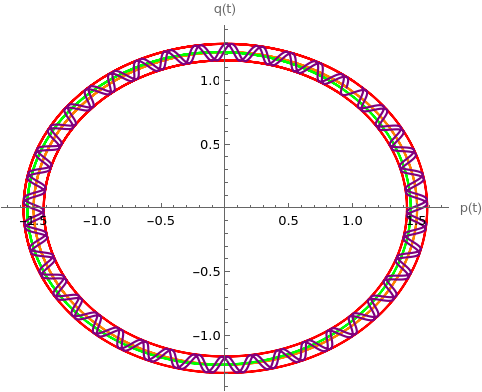
\includegraphics[width=9.0cm]{phase3.png}
  \caption{Possible Microstates}
\end{figure}
You may not be able to distinguish them but here is a brief description:
\begin{itemize}
\item Orange: An ellipse concentric with the other two red ones:
\item Green: An ellipse shifted to the left a bit, but still within the boundary of the two red ones
\item Purple: An ellipse whose radius oscillates but still maintains an energy within the bounds of the red ellipses
\end{itemize}
\subsection{Probability Distribution}
In equilibrium, the evolution of the probability is stable, so we have:
\begin{align*}
  \PB{\rho_{eq}}{H}=0
\end{align*}
Writing out the Poisson bracket:
\begin{align*}
  \PB{\rho_{eq}}{H}=\pdv{\rho_{eq}}{q}\pdv{H}{p}-\pdv{\rho_{eq}}{p}\pdv{H}{q}
\end{align*}
Using the Hamiltonian we get is:
\begin{align*}
  \pdv{H}{p}&=\frac{p}{m}\\
  \pdv{H}{q}&=kq
\end{align*}
The differential equation we need to solve is then:
\begin{align*}
  \pdv{\rho_{eq}}{q}\frac{p}{m}-\pdv{\rho_{eq}}{p}kq=0
\end{align*}
This is a separable partial differential equation, which we can see by:
\begin{align*}
  \pdv{\rho_{eq}}{q}\frac{p}{m}-\pdv{\rho_{eq}}{p}kq&=0\\
  \pdv{\rho_{eq}}{q}\frac{1}{q}-\pdv{\rho_{eq}}{p}\frac{km}{p}&=0
\end{align*}
Separating using $\rho_{eq}(p,q)=\mathcal{Q}(q)\mathcal{P}(p)$:
\begin{align*}
  \pdv{\rho_{eq}}{q}\frac{1}{q}-\pdv{\rho_{eq}}{p}\frac{km}{p}=
  \dv{\mathcal{Q}}{q}\frac{\mathcal{P}}{q}
  -\dv{\mathcal{P}}{p}\frac{km}{p}\mathcal{Q}&=0\\
  =\dv{\mathcal{Q}}{q}\frac{1}{q\mathcal{Q}}
  -\dv{\mathcal{P}}{p}\frac{km}{p\mathcal{P}}&=0
\end{align*}
Using separation constant $-\alpha$, we have the following equations:
\begin{align*}
  \dv{\mathcal{Q}}{q}\frac{1}{q\mathcal{Q}}&=-\alpha\qquad
  \dv{\mathcal{P}}{p}\frac{km}{p\mathcal{P}}=-\alpha
\end{align*}
Which are standard linear differential equations:
\begin{align*}
  \dv{\mathcal{Q}}{q}&=-\alpha q\mathcal{Q}\qquad
  \dv{\mathcal{P}}{p}=-\frac\alpha{km}p\mathcal{P}
\end{align*}
These both have Gaussian solutions, giving overall solutions:
\begin{align*}
  \rho_{eq}=A\exp{-\alpha\qty(q^2+\frac{p^2}{km})}
\end{align*}
We can determine the constant $A$ using the normalization:
\begin{align*}
  \int_{-\infty}^\infty\int_{-\infty}^\infty\dd{p}\dd{q}\rho_{em}=1
\end{align*}
The gaussian integral is standard, so we can get:
\begin{align*}
  \int_{-\infty}^\infty\int_{-\infty}^\infty\dd{p}\dd{q}\rho_{em}=
  \frac{A\pi}{\alpha}\sqrt{km}
\end{align*}
Thus the probability Distribution is:
\begin{align}
  \boxed{
    \rho_{eq}=\frac{\alpha}{\pi\sqrt{km}}\exp{-\alpha\qty(q^2+\frac{p^2}{km})}
  }
\end{align}
\section{One Dimensional Gas}
\subsection{Density from Liouville Equation}
We want to find $\rho(q,p,t)$, We know from Liouville's Equation:
\begin{align*}
  \pdv{\rho}{t}=-\PB{\rho}{H}
\end{align*}
Hamiltonian in this case is:
\begin{align*}
  H=\frac{p^2}{2m}
\end{align*}
Since it is a 1-D trap it is confined to only $x$, but it is a free particle in that degree of freedom, hence why it is a scalar $p^2$. The Poisson Bracket simplifies since:
\begin{align*}
  \pdv{H}{q}=0\qquad\pdv{H}{p}=\frac{p}{m}
\end{align*}
Hence we need to solve:
\begin{align*}
  \pdv{\rho}{t}=-\frac{p}{m}\pdv{\rho}{q}
\end{align*}
We can replace the solution at time $t$ with the solution at $t=0$ adjusted by the generalized velocity times $t$:
\begin{align*}
  \rho(q,p,t)=\rho\qty(q-\frac{p}{m}t,0)
\end{align*}
Which makes sense since we know it will act like a free particle. As for the momentum part, we need the boundary condition, specifically on $p$, since we are given none regarding it, hence we can multiply our solution by it to get the same information as it will cancel on either side, giving our solution:
\begin{align}
  \boxed{\rho(q,p,t)=\frac1{\sqrt{2\pi mk_bT}}
  \delta\qty(q-\frac{p}mt)\exp{-\frac{p^2}{2mk_bT}}}
\end{align}
Which, when we plot in phase space gives:
\begin{figure}[H]
  \centering
  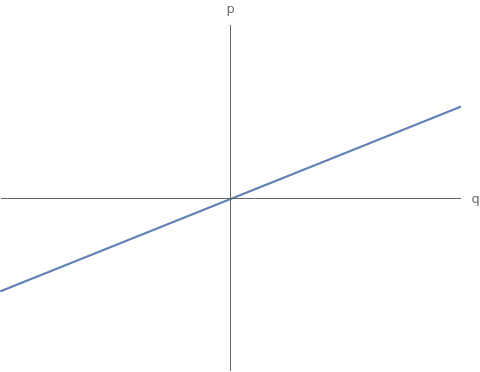
\includegraphics[width=8.0cm]{phase4.png}
  \caption{Phase Space}
\end{figure}
The plot is a line with slope m/t due to the delta function which relates the two
\subsection{Average Position and Momentum Squared}
Each average is given by an integral:
\begin{align*}
  \ev{q^2}&=\int_{PS}\dd{p}\dd{q}q^2\rho(q,p,t)=\frac1{\sqrt{2\pi mk_bT}}
  \int_{-\infty}^\infty\dd{p}\exp{-\frac{p^2}{2mk_bT}}
  \int_{-\infty}^\infty\dd{q}q^2\delta\qty(q-\frac{p}{m}t)\\
  \ev{p^2}&=\int_{PS}\dd{p}\dd{q}p^2\rho(q,p,t)=\frac1{\sqrt{2\pi mk_bT}}
  \int_{-\infty}^\infty\dd{p}p^2\exp{-\frac{p^2}{2mk_bT}}
  \int_{-\infty}^\infty\dd{q}\delta\qty(q-\frac{p}{m}t)
\end{align*}
Both of the $q$ integrals are fairly simple using the definition of the delta function:
\begin{align*}
  \int_{-\infty}^\infty\dd{q}q^2\delta\qty(q-\frac{p}{m}t)&=
  \qty(\frac{pt}{m})^2\\
  \int_{-\infty}^\infty\dd{q}\delta\qty(q-\frac{pt}{m}t)&=
  1
\end{align*}
Thus the remaining momentum integrals are:
\begin{align*}
  \ev{q^2}&\propto\frac{t^2}{m^2}
  \int_{-\infty}^\infty\dd{p}p^2\exp{-\frac{p^2}{2mk_bT}}\\
  \ev{p^2}&\propto
  \int_{-\infty}^\infty\dd{p}p^2\exp{-\frac{p^2}{2mk_bT}}
\end{align*}
These are essentially the same integral, which can be solved by integrating by parts twice and using the Standard Gaussian Integral:
\begin{align*}
  \int_{-\infty}^\infty\dd{p}p^2\exp{-\frac{p^2}{2mk_bT}}
  =\sqrt{2\pi}\qty(mk_bT)^{3/2}
\end{align*}
With the prefactor we had before we can reduce this to:
\begin{align*}
  \ev{p^2}=\frac{\sqrt{2\pi}\qty(mk_bT)^{3/2}}{\sqrt{2\pi mk_bT}}=
  mk_bT
\end{align*}
And the average square position is proportional to this:
\begin{align*}
  \ev{q^2}=\frac{t^2}{m^2}\ev{p^2}=\frac{k_bTt^2}{m}
\end{align*}
Giving the answers:
\begin{equation}
  \boxed{
  \begin{aligned}
    \ev{p^2}&=mk_bT\\
    \ev{q^2}&=\frac{k_bTt^2}{m}
  \end{aligned}}
\end{equation}
\subsection{Inserting Hard Walls}
To get a relaxation time, we need a length and a velocity. The velocity here should be defined by the average momentum over m, however the average momentum is $0$. We instead should use the square root of the average momentum squared over m instead:
\begin{align*}
  v_{c}=\frac{\sqrt{\ev{p^2}}}{m}
\end{align*}
The characteristic length should just be the length of the box, the distance between the walls at $\pm Q$, aka $2Q$, giving a relaxation time of:
\begin{align*}
  \tau=\frac{L}{v_c}\approx\frac{2Q}{\frac{\sqrt{\ev{p^2}}}{m}}
\end{align*}
This can be simplified to:
\begin{align}
  \boxed{\tau\approx2Q\sqrt{\frac{m}{k_bT}}}
\end{align}
Since the walls are hard, they act in such a way that whenever a collision happens, the momentum completely shifts negative for the particle upon a collision. So the phase space diagram becomes a sort of sideways shifted sawtooth wave. 
\subsection{Coarse Grained Density}
Eventually the slope of the line will diminish since the slope is inversely proportional to $t$. After $t>\tau$, or even much greater than it, a great many lines will pass through a coarse grained section of phase space. Eventually it will look like:
\begin{align*}
  \tilde{\rho}=\frac{f(p)}{2Q}
\end{align*}
The likelihood of any position is uniform it is just one over the interval length, and the momentum density is unchanged by the Liouville equation. Note that is is neither position nor time independent, so the Liouville equation reads:
\begin{align*}
  \pdv{\tilde{\rho}}{t}&=0\\
  -\frac{p}{m}\pdv{\tilde{\rho}}{q}&=0
\end{align*}
Thus we can say:
\begin{align}
  \boxed{\tilde{\rho}\text{ is stationary}}
\end{align}
\section{Evolution of Entropy}
\subsection{Liouville to Entropy}
The time derivative of the given entropy is:
\begin{align*}
  \dv{S}{t}&=-\dv{t}\int\dd{PS}\rho\ln\rho
  =-\int\dd{PS}\pdv{t}\qty(\rho\ln\rho)\\
  &=-\int\dd{PS}\qty(\ln\rho\pdv{\rho}{t}+\pdv{\rho}{t})\\
  &=-\int\dd{PS}\pdv{\rho}{t}\qty(\ln\rho+1)
\end{align*}
Where $PS$ is meant to represent all phase space variables.

Using Liouville's theorem we can interchange the time derivative of $\rho$ with derivatives with respect to coordinates:
\begin{align*}
  \dv{S}{t}=-\int\dd{PS}\sum_{i=1}^N\qty(\pdv{\rho}{\vb{p}}\vdot\pdv{H}{\vb{q}}
  -\pdv{\rho}{\vb{q}}\pdv{H}{\vb{p}})\qty(\ln\rho+1)
\end{align*}
If we separate these two terms and integrate them both by parts, assuming boundary terms go away:
\begin{align*}
  \dv{S}{t}=\int\dd{PS}\sum_{i=1}^N\qty(
  \rho\pdv{\vb{p}}\vdot\qty[\pdv{H}{\vb{q}}\qty(\ln\rho+1)]
  -\rho\pdv{\vb{q}}\vdot\qty[\pdv{H}{\vb{p}}\qty(\ln\rho+1)])
\end{align*}
The derivatives written out are:
\begin{align*}
  \pdv{\vb{p}}\vdot\qty[\pdv{H}{\vb{q}}\qty(\ln\rho+1)]=
  \pdv{H}{\vb{p}}{\vb{q}}\qty(\ln\rho+1)
  +\frac1\rho\pdv{H}{\vb{q}}\vdot\pdv{\rho}{\vb{p}}\\
  \pdv{\vb{q}}\vdot\qty[\pdv{H}{\vb{p}}\qty(\ln\rho+1)]=
  \pdv{H}{\vb{q}}{\vb{p}}\qty(\ln\rho+1)
  +\frac1\rho\pdv{H}{\vb{p}}\vdot\pdv{\rho}{\vb{q}}\\
\end{align*}
Notice the second derivatives of the Hamiltonian have opposite signs in the total expression and we are left with:
\begin{align*}
  \int\dd{PS}\sum_{i=1}^N\qty(\pdv{H}{\vb{q}}\vdot\pdv{\rho}{\vb{p}}
  -\pdv{H}{\vb{p}}\vdot\pdv{\rho}{\vb{q}})
\end{align*}
Integrating by parts again and using the fact that the mixed partials are equal, this gives:
\begin{align}
  \boxed{\dv{S}{t}=0}
\end{align}
\subsection{Maximizing Entropy}
We have two constraints, one associated with Lagrange multiplier $\alpha$:
\begin{align*}
  \int\dd{PS}\rho=1
\end{align*}
And one associated with Lagrange multiplier $\beta$:
\begin{align*}
  E=\int\dd{PS}\rho H
\end{align*}
The Entropy function we need to maximize is:
\begin{align*}
  S(t)=\int\dd{PS}\rho\qty[-\ln\rho-\alpha-\beta H]+\alpha+\beta E
\end{align*}
Performing the variational derivative:
\begin{align*}
  0=-\ln\rho_m-\alpha-\beta H-1
\end{align*}
Solving for $\rho_m$:
\begin{align*}
  \rho_m=e^{-(\alpha+1)-\beta H}
\end{align*}
\subsection{Stationary Solution}
From Liouville's equation, the Poisson Bracket of $\rho_m$ with $H$ is going to be proportional to:
\begin{align*}
  \PB{\rho_m}{H}\propto\PB{e^{-\beta H}}{H}
\end{align*}
The derivative of an exponential is proportional to the derivative of the argument, this should be $0$:
\begin{align*}
  \PB{e^{-\beta H}}{H}=\pdv{H}{p}\pdv{H}{q}e^{-\beta H}
  -\pdv{H}{q}\pdv{H}{p}e^{-\beta H}=0
\end{align*}
Hence:
\begin{align}
  \boxed{\pdv{\rho_m}{t}=-\PB{\rho_m}{H}=0}
\end{align}
\subsection{Making Sense of This}
Even though the probability density is changing, it is doing in a way that preserves information content, which is why $S(t)$ is not increasing. However, as time goes on, the probability disperses a bit, which means the information content is lower, which is what we mean by maximum entropy
\end{document}